\marginpar{VL am 13.05.19}
\subsubsection{Netzdynamik} \label{sec:netzdynamik}
$\hat{=}$ Markenfluss im PN, bewirkt durch \textit{Schaltvorgänge} aktivierter Transitionen \beiblatt{2-8}

\properparagraph{Beispiel}
\underline{kein Schaltvorgang}

\begin{figure}[H]
	\centering
	\includegraphics[width=0.25\textwidth]{img/2019_05_13/abb1.tikz}
\end{figure}
\begin{itemize}
	\item \textcolor{green}{$t_1$ nicht aktiv ( 1) nicht erfüllt)}
	\item \textcolor{blue}{$t_1$ nicht aktiv ( 1) nicht erfüllt)}
\end{itemize}

\underline{Schaltvorgang}
$t_1$ aktiv $\rightarrow$ Schaltvorgang

\begin{figure}[H]
	\centering
	\subfloat[]{\includegraphics[width=0.25\textwidth]{img/2019_05_13/abb2.tikz}} \qquad $\Rightarrow$ \qquad
	\subfloat[]{\includegraphics[width=0.25\textwidth]{img/2019_05_13/abb4.tikz}}
\end{figure}


\underline{Kontakt}

\begin{figure}[H]
	\centering
	\includegraphics[width=0.25\textwidth]{img/2019_05_13/abb3.tikz}
\end{figure}
\begin{itemize}
	\item \textcolor{green}{$t_1$ nicht aktiv ( 2) nicht erfüllt)}
	\item \textcolor{blue}{$t_1$ nicht aktiv ( 2) nicht erfüllt)}
	\item \textcolor{red}{$t_1$ nicht aktiv ( 2) nicht erfüllt)}
\end{itemize}

\underline{Konflikt}
\begin{figure}[H]
	\centering
	\subfloat[Alternative]{\includegraphics[width=0.25\textwidth]{img/2019_05_13/abb5.tikz}} \qquad \qquad \qquad
	\subfloat[Begegnung]{\includegraphics[width=0.25\textwidth]{img/2019_05_13/abb6.tikz}}
\end{figure}


\properparagraph{Konfliktlösung (mittels Zusatzwissen)}
\begin{itemize}
	\item Zusätzliche bool'sche Bedingung an den Transitionen
	\item Kantenzeitbewertung (siehe später)
	\item Alternierendes Schalten
	\item Zufallsauswahl
\end{itemize}

\properparagraph{Demo: DESSKA}
%TODO Abb.

\subsubsection{Netzklassen}
\underline{Netzklassen:} Netz mit bestimmten (beschränkten) Eigenschaften zur Abbildung der jeweils charakteristischen dynamischen Abläufe (Beschränkung vorteilhaft für die Analyse/Synthese).

Klassifizierung nach:
\begin{itemize}
	\item Struktureigenschaften
	\item Stellen-/Kanteneigenschaften 
	\smash{\raisebox{.5\dimexpr1\baselineskip+4\itemsep+2\parskip}{$\left.\rule{0pt}{.5\dimexpr2\baselineskip+3\itemsep+3\parskip}\right\}\text{\beiblatt{2-9, 2-10}}$}} 
\end{itemize}

\properparagraph{Erläuterungen Struktureigenschaften}
\begin{itemize}
	\item \textbf{\underline{Reines PN}}
	
	Schleifen verboten
	\begin{figure}[H]
		\centering
		\includegraphics[width=0.25\textwidth]{img/2019_05_13/abb7.tikz}
	\end{figure}
	
	\item \textbf{\underline{Zustandsmaschine (ZM)}}
	
	Beispiel:
	\begin{figure}[H]
		\centering
		\includegraphics[width=0.5\textwidth]{img/2019_05_13/abb8.tikz}
	\end{figure}
	
	Kennzeichen:
	\begin{itemize}
		\item Abbildung alternativer Abläufe
		\item Markenzahl in ZM konstant
		\item Markenanzahl:
		\begin{itemize}
			\item mehrere Marken: Nebenläufigkeit darstellbar (aber: $\forall s_i: K(s_i)>1$ erforderlich)
			\item genau eine Marke: ZM $\hat{=}$ Automatengraph
		\end{itemize}
	\end{itemize}

	\item \underline{Synchronisationsgraph (SG)} (s. \textit{BB AEH 2-10})
	
	Beispiel:
	\begin{figure}[H]
		\centering
		\includegraphics[width=0.5\textwidth]{img/2019_05_13/abb9.tikz}
	\end{figure}
	
	Kennzeichen:
	\begin{itemize}
		\item Modellierung von Nebenläufigkeit
		\item Keine Alternativen abbildbar (dadurch konfliktfrei)
		\item Markenzahl nicht konstant
	\end{itemize}

	\item \underline{Free-Choice-Netze (FC-Netz)} (s. \textit{BB AEH 2-10})
	
	Kennzeichen:
	\begin{itemize}
		\item Kombination von ZM- und SG-Strukturen \newline ($\Rightarrow$ ZM $\subset$ FC-Netz, SG $\subset$ FC-Netz)
		\item bei Alternativen ist nur der Ausgangszustand (Konfliktstelle) betroffen, kein Einfluss anderer Zustände (Stellen)
	\end{itemize}
\end{itemize}

\properparagraph{Anmerkungen}
\begin{enumerate}
	\item Erweiterung des FC-Netz: \underline{Extended Free-Choice-Netz (EFC-Netz)}
	
	Gegenseitig bedingte Alternativen zulässig
	\begin{figure}[H]
		\centering
		\includegraphics[width=0.25\textwidth]{img/2019_05_13/abb10.tikz}
	\end{figure}
	
	\item allgemeinstes PN: \underline{Stellen/Transitionen-Netz (S/T-Netz)}
	
	Alle Struktur- und Knoten/Kanteneigenschaften erlaubt (demzufolge alle übrigen Netzklassen).
\end{enumerate}

\properparagraph{Beispiel 1}
\begin{figure}[H]
	\centering
	\includegraphics[width=\textwidth]{img/2019_05_13/abb11.tikz}
\end{figure}

\begin{itemize}
	\item ZM: nein, da z.B. $|t_4 \bullet| = 2$
	\item SG: nein, da z.B. $|s_1 \bullet| = 2$
	\item FC-Netz:
	\begin{equation}
		|s_i \bullet| = 1 \qquad \forall i=2,\,\ldots,\,4
	\end{equation}
	\begin{equation}
	s_1 \bullet = \{t_1,\,t_3\},\quad \bullet (s_1 \bullet) = \bullet t_1 = \{s_1\} = \bullet t_3
	\end{equation}
	$\Rightarrow$ ja!  
\end{itemize}

\textcolor{blue}{Kein gewöhnliches PN $\Rightarrow$ S/T Netz}

\properparagraph{Beispiel 2}
\begin{figure}[H]
	\centering
	\includegraphics[width=\textwidth]{img/2019_05_13/abb11.tikz}
\end{figure}

Ohne Konfliktlösung:
\begin{itemize}
	\item ZM: ja
	\item SG: nein, da z.B. $|s_1 \bullet| = 2$
	\item FC: ja
\end{itemize}

\textcolor{blue}{Mit Konfliktlösung:}
\begin{figure}[H]
	\centering
	\includegraphics[width=0.5\textwidth]{img/2019_05_13/abb12.tikz}
\end{figure}
\begin{itemize}
	\item ZM: nein, da z.B. $|\bullet t_1|=2$
	\item FC-Netz:
	\begin{align}
		(s_1 \bullet) &= \{t_1,\,t_2\} \\
		\bullet(s_1 \bullet) &= \bullet t_1 = \{s_1,\,s_3\} \\
		\bullet t_2 &= \{s_1,\,s_4\}
	\end{align}
	$\Rightarrow$ nein
\end{itemize}
	$\Rightarrow$ S/T-netz

\includepdf[pages={18 - 20}]{material/AEH_2019.pdf}